\chapter{QAOA for Max-Cut}
The aim of the \gls{maxcut} problem is to find a set of vertices that maximizes the sum of the weights of the edges that are cut.
It is a widely studied problem known to be $\NP$-hard.
Formally, given an undirected graph $G = (V, E)$ with $n = |V|$ vertices and non-negative weights $w_{j, k} = w_{k, j}$ on the edges $(j, k) \in E$, one looks to bipartition $V$ into two sets $S \subseteq V$ and $\bar{S} = V \setminus S \subseteq V$ such that the objective function $L$ is maximized:
\begin{equation} \label{eqn:max-cut-objective}
L(z) = \sum_{(j, k) \in E} w_{j, k}[z_j(1 - z_k) + z_k(1 - z_j)].
\end{equation}
Here $z \in \{0, 1\}^n$ is a bit string that describes the bipartition as follows: if a vertex $j$ is in partition $S$, then $z_j = 0$, and if a vertex $j$ is in partition $\bar{S}$ then $z_j = 1$.
For example, \Cref{fig:maxcut-5-example} shows an example of a maximum cut on a graph with five vertices.
The partition of that cut can be described as the bit string $z = 00101$.
\begin{figure}[ht]
    \centering
    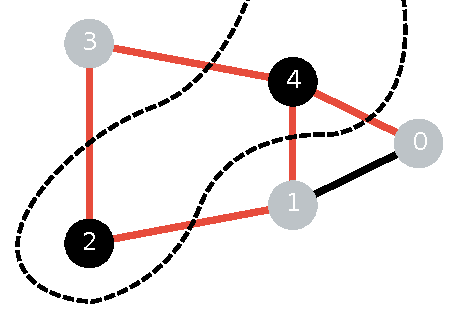
\includegraphics[width=0.4\linewidth]{figures/maxcut_5_graph_cut_example.pdf}
    \caption[\Gls{maxcut} example on a graph with five vertices and unit weights.]{
        \Gls{maxcut} example on a graph with five vertices and unit weights.
        The vertices are partitioned into two sets visualized as black and gray.
        The cut shown is a maximum cut with $L(z) = 5$, which can be thought of as the number of edges cut (shown in red).
    }
    \label{fig:maxcut-5-example}
\end{figure}

The \gls{qaoa} algorithm can be used for solving \gls{maxcut} problems by assigning a vertex $j \in V$ to a qubit $\ket{q_j}$.
A qubit $\ket{q_j}$ is in state \ket{0} if a vertex $j$ is in partition $S$, and state \ket{1} if vertex $j$ is in partition $\bar{S}$.
To encode the objective function from \Cref{eqn:max-cut-objective}, note that the objective function can be rewritten as follows:
\begin{equation}
L(z) = \frac{1}{2} \sum_{(j, k) \in E} w_{j, k}(1 - z_jz_k),
\end{equation}
where $z_j \in \{-1, 1\}$ for $j \in V$.
This objective function can be represented by the following problem Hamiltonian:
\begin{equation} \label{eqn:problem-hamiltonian}
H_L = \frac{1}{2} \sum_{(j, k) \in E} w_{j, k}(I - Z^{(j)}Z^{(k)}).
\end{equation}
This gives the problem unitary
\begin{equation} \label{eqn:problem-unitary}
U_L(\gamma) = e^{-i\gamma H_L} = \prod_{(j, k) \in E} e^{-i\gamma w_{j, k}(I - Z^{(j)}Z^{(k)})/2},
\end{equation}
and the standard mixer unitary as defined in \Cref{sec:qaoa}:
\begin{equation} \label{eqn:mixer-unitary}
U_B(\beta) = e^{-i\beta H_B} = \prod_{j \in V} e^{-i\beta X^{(j)}}.
\end{equation}

\section{Implementation}
The \gls{qaoa} was implemented in Python using the Project Q~\cite{steiger2018projectq}, Quantum Inspire~\cite{quantuminspire}, and SciPy~\cite{scipy} frameworks to solve the \gls{maxcut} problem on the graph from \Cref{fig:maxcut-4-graph}.
The optimal solutions for this graph are $z = 0101$ and $z = 1010$ with $L(z) = 4$.
\begin{figure}[ht]
    \centering
    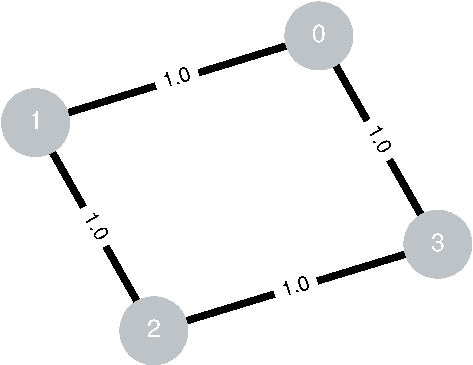
\includegraphics[width=0.4\linewidth]{figures/maxcut_4_graph.pdf}
    \caption{
        Undirected 2-regular graph $G = (V, E)$ with $n = 4$ vertices $V = \{0, 1, 2, 3\}$ and 4 edges $E = \{(0,1), (0,3), (1,2), (2,3)\}$ with unit weight $w_{j, k} = w_{k, j} = 1$.
    }
    \label{fig:maxcut-4-graph}
\end{figure}
A $ZZ$ interaction $e^{-i\gamma w_{j, k}(I - Z^{(j)}Z^{(k)})/2}$ from the problem unitary $U_L(\gamma)$ (\Cref{eqn:problem-unitary}) is implemented as follows:
\begin{figure}[H]
    \[
    \Qcircuit @C=1em @R=1em @!R {
        & \lstick{\ket{q_j}} & \ctrl{1} & \qw & \ctrl{1} & \qw \\
        & \lstick{\ket{q_k}} & \targ & \gate{R_z(-\gamma w_{j, k})} & \targ & \qw
    }
    \]
\end{figure}
\noindent
The $X$ interaction $e^{-i\beta X^{(j)}}$ from the mixer unitary $U_B(\beta)$ (\Cref{eqn:mixer-unitary}) is implemented as a $R_x$ gate:
\begin{figure}[H]
    \[
    \Qcircuit @C=1em @R=1em @!R {
        & \lstick{\ket{q_j}} & \gate{R_x(2\beta)} & \qw \\
    }
    \]
\end{figure}
\noindent
The complete quantum circuit for the \gls{qaoa} for \gls{maxcut} on this graph is shown in \Cref{fig:qaoa-circuit}.

The quantum circuit is implemented using the Qiskit quantum computing library.
To find the optimal parameters $\vec{\gamma}^*, \vec{\beta}^*$ a classical optimizer provided by SciPy is used.
The relevant cost function is
\begin{equation}
C_p(\vec{\gamma}, \vec{\beta}) = \bra{\psi(\vec{\gamma}, \vec{\beta})}H_L\ket{\psi(\vec{\gamma}, \vec{\beta})},
\end{equation}
and we look to solve the optimization problem
\begin{equation}
\vec{\gamma}^*, \vec{\beta}^* = \argmax_{\vec{\gamma}, \vec{\beta}} C_p(\vec{\gamma}, \vec{\beta}).
\end{equation}
We then prepare the state $\ket{\psi(\vec{\gamma}^*, \vec{\beta}^*)}$ and measure multiple times in the computational basis to extract the solution, which is the bit string with the highest probability.

\begin{figure}
    \begin{adjustwidth}{-1cm}{-1cm}
    \[
    \Qcircuit @C=0.275em @R=0.8em @!R {
        & & & & & \lstick{\ket{q_0}} & \gate{H} & \qw & \ctrl{1} & \qw & \ctrl{1} & \qw & \ctrl{3} & \qw & \ctrl{3} & \qw & \qw & \qw & \qw & \qw & \qw & \qw & \qw & \qw & \gate{R_x(2\beta)} & \qw & \qw & \meter & \cw \\
        & & & & & \lstick{\ket{q_1}} & \gate{H} & \qw & \targ & \gate{R_z(-\gamma w_{0, 1})} & \targ & \qw & \qw & \qw & \qw & \qw & \ctrl{1} & \qw & \ctrl{1} & \qw & \qw & \qw & \qw & \qw & \gate{R_x(2\beta)} & \qw & \qw & \meter & \cw \\
        & & & & & \lstick{\ket{q_2}} & \gate{H} & \qw & \qw & \qw & \qw & \qw & \qw & \qw & \qw & \qw & \targ & \gate{R_z(-\gamma w_{1, 2})} & \targ & \qw & \ctrl{1} & \qw & \ctrl{1} & \qw & \gate{R_x(2\beta)} & \qw & \qw & \meter & \cw \\
        & & & & & \lstick{\ket{q_3}} & \gate{H} & \qw & \qw & \qw & \qw & \qw & \targ & \gate{R_z(-\gamma w_{0, 3})} & \targ & \qw & \qw & \qw & \qw & \qw & \targ & \gate{R_z(-\gamma w_{2, 3})} & \targ & \qw & \gate{R_x(2\beta)} \gategroup{1}{9}{4}{25}{1em}{--} & \qw & \qw & \meter & \cw \\
        & & & & & & & & & & & & & \hspace{5cm} p \mbox{ times}
    }
    \]
    \end{adjustwidth}
    \caption[Quantum circuit for the $p$-layer \gls{qaoa} on the graph from \Cref{fig:maxcut-4-graph}.]{
        Quantum circuit for the $p$-layer \gls{qaoa} on the graph from \Cref{fig:maxcut-4-graph}.
        Each vertex $j \in V$ is represented by qubit $\ket{q_j}$.
        The circuit starts by preparing an equal superposition state, after which the problem unitary $U_L(\gamma)$ and mixer unitary $U_B(\beta)$ are applied $p$ times.
        In general, the depth of the circuit is $p(3m + n)$, where $p$ is the number of layers, $m$ is the number of edges, and $n$ is the number of vertices. 
    }
    \label{fig:qaoa-circuit}
\end{figure}

\section{Results}
The implementation from the previous section is run on two different Quantum Inspire back-ends: the QX simulator back-end and the Starmon-5 \gls{qpu} back-end.
The cost function is optimized for 30 iterations using the \gls{cobyla} algorithm.
For the quantum circuit executions during optimization 1024 shots were used, and for the final measurement 4096 shots were used.
The results from the experiments are shown in \Cref{fig:qaoa-results}.
The QX simulator back-end manages to find a local minimum with a final approximation ratio of $0.76$ and high probabilities of measuring the optimal solutions $z = 1010$ and $z = 0101$.
The Starmon-5 \gls{qpu} back-end reaches a final approximation ratio of $0.63$ and manages to reach a final state which measures an optimal solution $z = 0101$ with high probability.
The performance difference between the simulator and \gls{qpu} back-end was expected: while \glspl{hqca} have some robustness against noise, their performance on real hardware will still be significantly worse from idealized noise-free simulations.
Further performance improvement could be achieved on \glspl{qpu} by choosing a classical optimizer that is more robust against noise as discussed in \cite{lavrijsen2020classical, sung2020exploration}, but such work is beyond the scope of this report.
Nonetheless, these experiments demonstrate the potential of quantum computers and even \gls{nisq} devices to solve practical problems in the near future.
While being far away from being more efficient than classical methods, such demonstration is an important step in the development of larger and better quantum computers.

\begin{figure}[ht]
    \centering
    \begin{subfigure}{.49\textwidth}
        \centering
        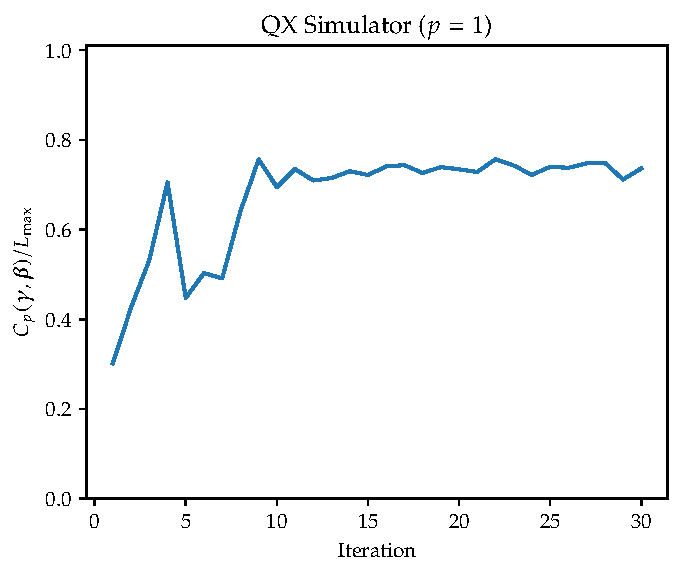
\includegraphics[width=1\linewidth]{figures/qaoa_maxcut_n4_p1_qx_optimization.pdf}
    \end{subfigure}
    \hfill
    \begin{subfigure}{.49\textwidth}
        \centering
        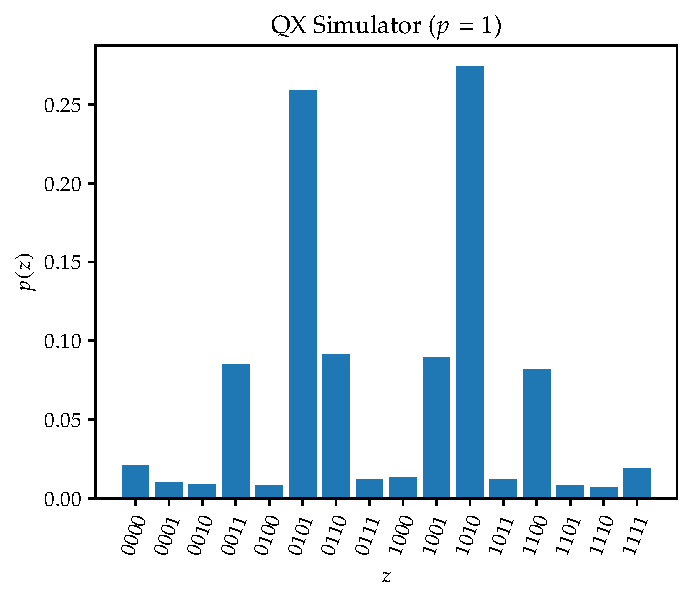
\includegraphics[width=1\linewidth]{figures/qaoa_maxcut_n4_p1_qx_probs.pdf}
    \end{subfigure}

    \begin{subfigure}{.49\textwidth}
        \centering
        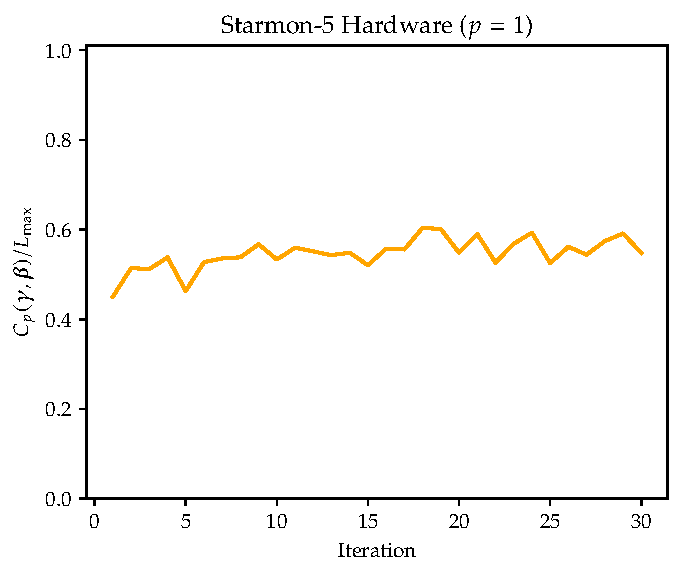
\includegraphics[width=1\linewidth]{figures/qaoa_maxcut_n4_p1_starmon_optimization.pdf}
    \end{subfigure}
    \hfill
    \begin{subfigure}{.49\textwidth}
        \centering
        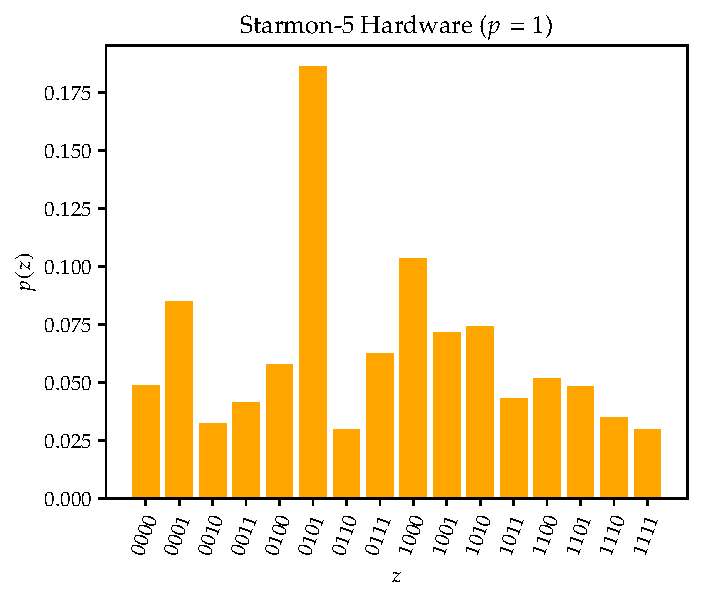
\includegraphics[width=1\linewidth]{figures/qaoa_maxcut_n4_p1_starmon_probs.pdf}
    \end{subfigure}

    \caption[Experimental results of the running the \gls{qaoa} to solve \gls{maxcut} problem on the graph from \Cref{fig:maxcut-4-graph}.]{
        Experimental results of the running \gls{qaoa} to solve the \gls{maxcut} problem on the graph from \Cref{fig:maxcut-4-graph}.
        The left column plots the approximation ratio $C_p(\vec{\gamma}, \vec{\beta})/L_\text{max}$ over 30 iterations, and the right column plots the final probabilities of measuring the possible solution bit strings after optimization.
        The top row contains results from the QX simulator back-end, and the bottom row contains the results from the Starmon-5 \gls{qpu} back-end.
    }
    \label{fig:qaoa-results}
\end{figure}